\section{Observation, event time, and completion}
\label{sec:observation}

\subsection{A feed is a projection}

CME's futures and options market-data documentation distinguishes market-by-price, market-by-order full-depth, and implied-book information \citep{CMEMDP}. A public view is written
\begin{equation}
 Y_n=\Pi(X_n).
\end{equation}
The map $\Pi$ can discard reserve size, unelected stops, account information, recipe inputs, or other attributes. An order identifier is not a participant identity. A full-depth order view does not imply full knowledge of the state in \eqref{eq:state}.

For the documented MBO view, ordering first uses instrument, side, and price, and then the order-priority value within the same price and side. Lower priority numbers rank ahead locally. The priority field is supplied regardless of the product's matching algorithm, and implied-book information is not transmitted in MBO format \citep{CMEMBO}. It follows that sorting an MBO book gives an observed order sequence; it does not convert every product into a FIFO allocation market.

\begin{proposition}[When an observed transition exists]\label{prop:projection}
Fix a deterministic event map $T_e$. There exists a map $\widetilde T_e$ on observed states with
\begin{equation}
 \Pi T_e=\widetilde T_e\Pi
\end{equation}
if and only if $\Pi T_e(x)=\Pi T_e(x')$ whenever $\Pi(x)=\Pi(x')$.
\end{proposition}
\begin{proof}
If $\widetilde T_e$ exists, equal observations have the same image under it. Conversely, define $\widetilde T_e(y)=\Pi T_e(x)$ for any $x$ with $\Pi(x)=y$. The stated condition makes this definition independent of the representative $x$.
\end{proof}

For a concrete failure, two books have the same price-level total ten and two orders. In one, order A has size two and order B size eight; in the other, A and B each have size five. Cancel A. Remaining price-level depth is eight in the first book and five in the second. Aggregated depth alone cannot determine the update even though the cancellation is unambiguous at order level.

A related failure occurs with hidden interest: two books may expose the same displayed order while carrying different reserves. Their observations can agree until a depletion event refreshes one of them. This does not contradict reconstruction of the displayed book; it limits what that reconstruction identifies.

\subsection{Complete events, not arbitrary message prefixes}

The CME event documentation groups messages generated by order actions and state changes, and provides the MatchEventIndicator to identify the event boundary. An event can include trades, book changes, and implied-quote changes; some events, such as entry of an unelected stop, need not produce public market data \citep{CMEEvents}.

Suppose a single matching event consumes an order that supports two implied quotes. An observer may receive a trade update, a direct-book update, and an implied update at different moments. A partial message prefix can temporarily combine a depleted direct order with its old implied quantities. Treating that prefix as a simultaneous executable state creates fictitious liquidity. Complete-event processing resolves this particular inconsistency, although it does not recover hidden state or eliminate network latency.

Let $\mathcal F_t^{\rm obs}$ be the information available after valid event completion and applicable recovery. A model should distinguish the last valid observation from an interval with an unresolved gap. Filling a sequence gap with a zero-change assumption creates data that were never observed. The numerical code accompanying this paper begins from synthetic complete states; it does not claim to decode MDP packets or implement recovery.

\subsection{The allocation map changes completion time}

To isolate allocation from order-arrival uncertainty, consider a static book repeatedly hit by same-price aggressors of fixed batch size $b$. Let the arrival count $N_t$ be a Poisson process with rate $\lambda>0$. At each arrival apply one declared allocation map, update remaining quantities, and continue. There are no competing orders or cancellations.

\begin{proposition}[An embedded-event completion law]\label{prop:erlang}
If order $i$ completes at deterministic arrival index $k_i$, then its completion time $T_i$ satisfies
\begin{equation}
 \Prob(T_i\le t)=\Prob(N_t\ge k_i)
 =1-e^{-\lambda t}\sum_{j=0}^{k_i-1}\frac{(\lambda t)^j}{j!},
 \qquad \E T_i=\frac{k_i}{\lambda}.
\end{equation}
\end{proposition}
\begin{proof}
Completion occurs exactly when the $k_i$th arrival has occurred. The Poisson count formula gives the distribution. Equivalently $T_i$ is the sum of $k_i$ independent exponential waiting times, each with mean $1/\lambda$.
\end{proof}

Return to $q=(12,28,60)$, batch size 37, and rate two events per second. Under FIFO, complete-fill indices are $(1,2,3)$, with means $(0.5,1,1.5)$ seconds. Under the $h=2$ pro-rata/FIFO model, the first two fills are both $(5,10,22)$; remaining quantities after the second are $(2,8,16)$. The third batch exhausts them. All complete-fill indices are three, with mean 1.5 seconds.

Every order receives a positive fill on the first pro-rata event, while the third FIFO order receives none on its first event. Yet early \emph{partial} participation does not imply earlier \emph{completion}. A fill-probability statistic must specify which event it measures.

\begin{figure}[htbp]
\centering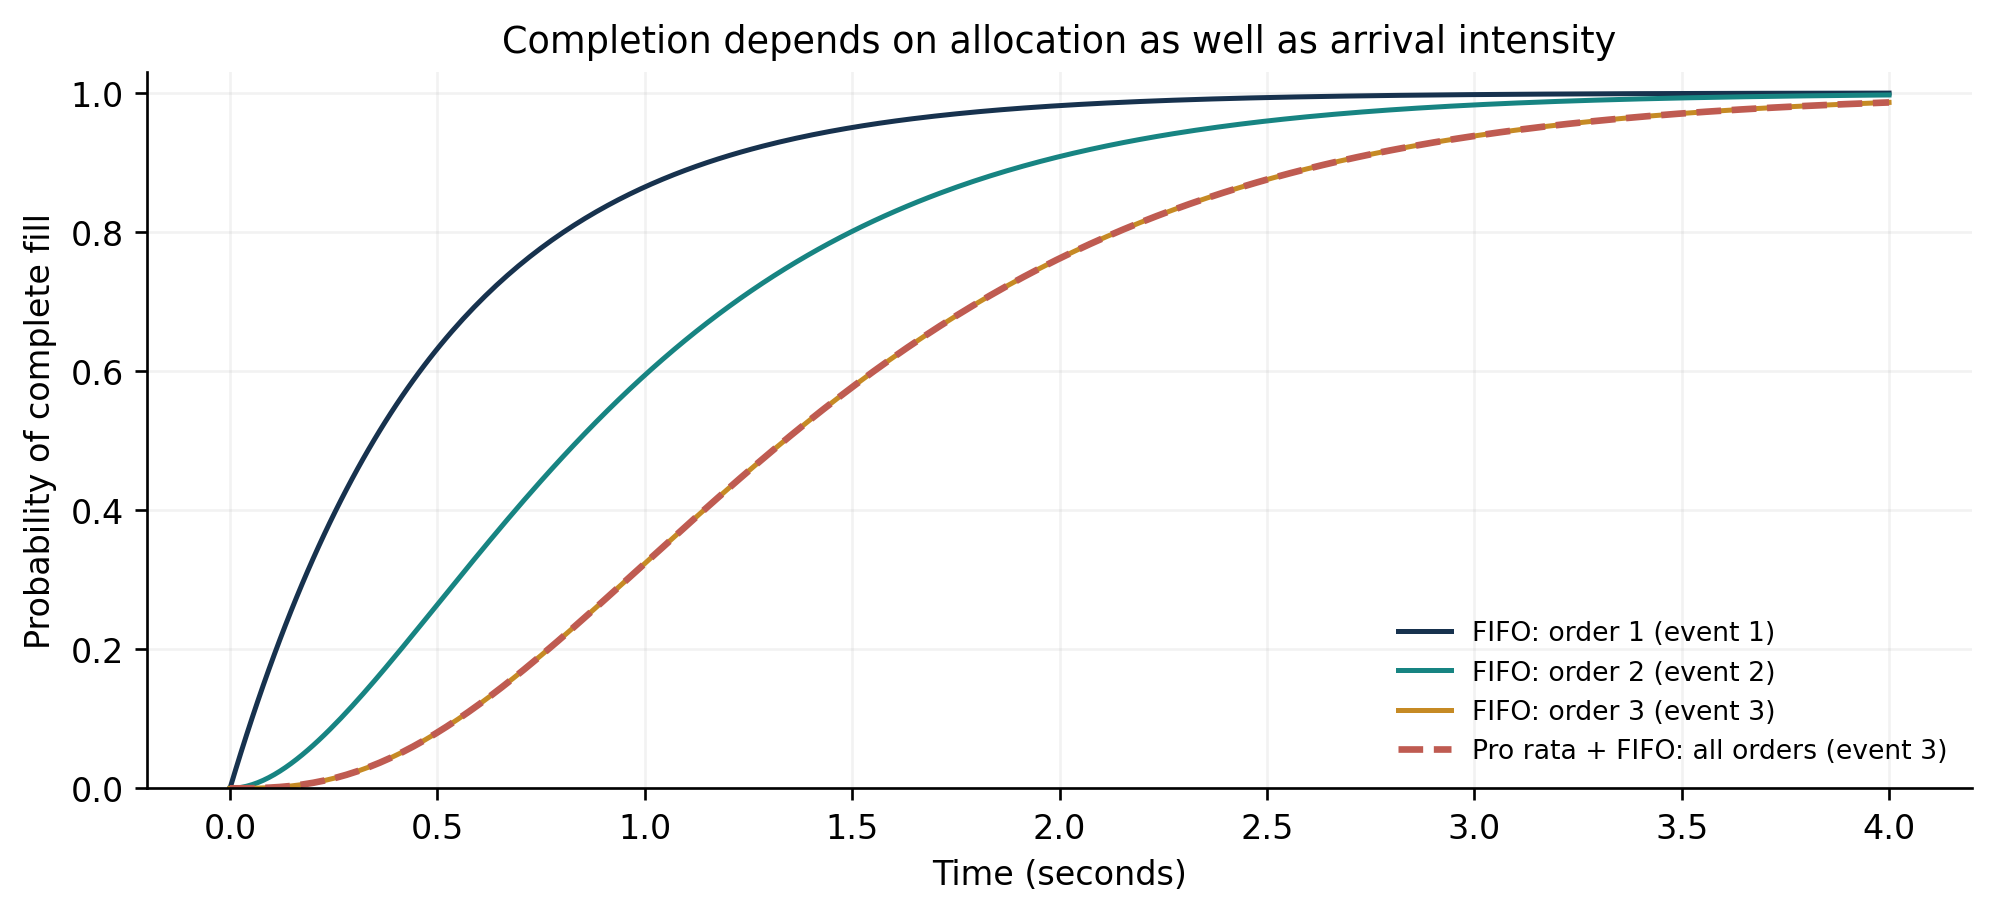
\includegraphics[width=.92\textwidth]{figures/04_completion.png}
\caption{Exact complete-fill distributions in the fixed-batch arrival model. The dashed curve coincides with the third FIFO curve because both require three arrivals. Arrival intensity is an illustrative assumption rather than an empirical estimate.}
\label{fig:completion}
\end{figure}

\subsection{Stochastic state and filtering}

A stochastic model can assign state-dependent intensities $\lambda_e(x)$ to events and generator
\begin{equation}
 (\mathcal Gf)(x)=\sum_e\lambda_e(x)[f(T_e x)-f(x)].
\end{equation}
Deterministic matching and random event arrivals then coexist without making the matching rule itself random. Price controls, cancellations, and replenishment require additional transitions. Queue depletion need not have an Erlang law under those extensions.

If the complete modeled state is Markov with transition matrix $P$ and observations are deterministic, a finite-state belief $\beta_n(x)$ updates through
\begin{equation}
 \beta_{n+1}(x')=
 \frac{\ind\{\Pi(x')=Y_{n+1}\}\sum_x\beta_n(x)P(x,x')}
 {\sum_{u:\Pi(u)=Y_{n+1}}\sum_x\beta_n(x)P(x,u)},
\label{eq:filter}
\end{equation}
when the denominator is positive. This expresses the difference between reconstructing observed messages and inferring unobserved state. A forecast of execution should condition on what was available at the decision time, not on subsequently repaired or future market data.
